\documentclass[../main.tex]{subfiles}




\begin{document}


\chapter{Homologia simplicial}


Aquest capítol és una introducció a l'homologia simplicial dels políedres. Hem vist en el capítol anterior com associar a un políedre qualsevol $K$ un enter $\chi(K)$, la característica d'Euler, però com podem compara les característiques d'Euler de diferents políedres? Si $f:|K|\rightarrow|L|$ és una aplicació contínua o, fins i tot, simplicial, la definició de $\chi$ no permet establir una relació entre $\chi(K)$ i $\chi(L)$. Veurem en aquest capítol que la característica d'Euler es pot calcular a partir dels grups d'homologia simplicial, i que l'aplicació simplicial $f$ indueix un morfisme dels grups d'homologia simplicial de $K$ en els de $L$. Això farà possible, en alguns casos, establir una relació entre $\chi(K)$ i $\chi(L)$.




\section{Cadenes d'un políedre. Homologia simplicial}


\begin{defi}[Símplex ordenat]
Si $\sigma = \langle v_0,\ldots,v_n\rangle$ és un símplex, diem que és un \textit{símplex ordenat}\index{Símplex ordenat} si hem fixat un ordre total en el conjunt de vèrtexs $\{v_0,\ldots,v_n\}$. Denotarem $[v_0,\ldots,v_n]$ un símplex ordenat tal que $v_0<v_1<\cdots<v_n$. Si $K$ és un complex simplicial, direm que és \textit{ordenat} si hem fixat un ordre total en $V_k$, és a dir, si $\forall \sigma\in K$ està ordenat.
\end{defi}

Intuïtivament, ordenar els vèrtexs d'un símplex és una forma d'orientar aquest símplex com mostra la figura \ref{fig:simplexsordenat}.
\begin{figure}
    \centering
    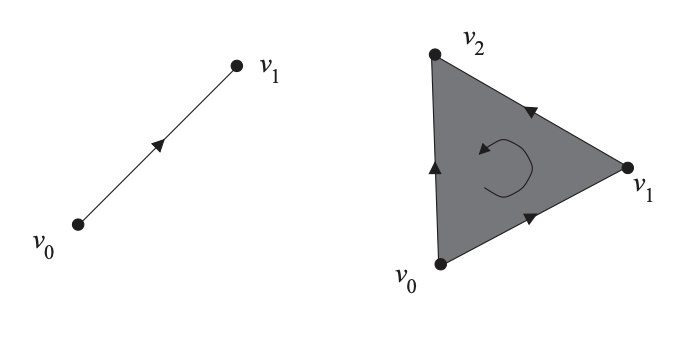
\includegraphics[scale = 0.25]{pictures/simplexsordenats.png}
    \caption{Símplexs ordenats}
    \label{fig:simplexsordenats}
\end{figure}

Al llarg d'aquest capítol, excepte si es diu el contrari, suposarem que els complexs simplicials que apareixen estan ordenats.


\begin{defi}[Grup de cadenes $p$-dimensionals]
Sigui $K$ un complex simplicial ordenat. Prenem l'anell $R = \mathbb{Z}$. Donat $p\geq 0$, anomenarem \textit{grup de cadenes $p$-dimensionals}\index{Grup de cadenes $p$-dimensionals} de $K$ a 
\begin{equation}
    \notag
    C_p(K) = \bigoplus_{\substack{\sigma\in K\\\dim\sigma=p\\\text{ordenat}}}\mathbb{Z}[\sigma] = \left\{
    \sum_{i=1}^n\lambda_i\sigma_i\;:\;\lambda_i\in\mathbb{Z},\;\sigma_i\;\text{símplex ordenat $p$-dimensional}
    \right\}
\end{equation}
és a dir, el grup abelià lliure generat pel conjunt de cares $p$-dimensionals ordenades
\end{defi}

Notem que si $p>\dim K$, aleshores $C_p(K) = 0$.

\begin{ej}
Si $K = [v_0,v_1,v_2]$, tenim
\begin{equation}
    \notag
    \begin{array}{ll}
        C_0(K) = \mathbb{Z}[v_0]\oplus\mathbb{Z}[v_1]\oplus\mathbb{Z}[v_2]\cong\mathbb{Z}^3\\
        C_1(K) = \mathbb{Z}[v_0,v_1]\oplus\mathbb{Z}[v_1,v_2]\oplus\mathbb{Z}[v_0,v_2]\cong\mathbb{Z}^3\\
        C_2(K)= \mathbb{Z}[v_0,v_1,v_2]\cong\mathbb{Z}
    \end{array}
\end{equation}
i, en general, per a un $n$-símplex, $\Delta^n$, tenim 
\begin{equation}
    \notag
    C_p(\Delta^n) \cong \mathbb{Z}^{\binom{n+1}{p+1}}\qquad p\leq n.
\end{equation}
\end{ej}

Les arestes $[v_0,v_1]$, $[v_0,v_2]$ i $[v_1,v_2]$ de l'exemple anterior formen la vora del $2$-símplex $\Delta^2$, si recorrem $[v_0,v_2]$ en sentit invers. L'operador vora que definirem a continuació és la versió algebraica d'aquest concepte geomètric. Observem, abans de donar aquesta definició, que com els grups de cadenes són grups abelians lliures, de base els símplexs de diferents dimensions, per definir un morfisme entre aquests grups és suficient definir-lo sobre les cares i estendre'l per linealitat.


\begin{defi}[Operador vora]\index{Operador vora}
Sigui $K$ complex simplicial ordenat. Donat $p\geq 1$, anomenarem \textit{operador vora} $\partial_p:C_p(K)\rightarrow C_{p-1}(K)$ al morfisme de grups que, sobre els generadors està definit per 
\begin{equation}
    \notag
    \partial_p([v_{i_0},\ldots,v_{i_p}]) = \sum_{k=0}^p(-1)^k[v_{i_0},\cdots,\hat{v}_{i_k},\ldots,v_{i_p}]
\end{equation}
on $\hat{v}_{i_k}$ vol dir que excloem el $v_{i_k}$.
\end{defi}

\begin{ej}
Per exemple, per un 1-símplex $\Delta^1 = [v_0,v_1]$ trobem
\begin{equation}
    \notag
    \begin{array}{rl}
        \partial_1:C_1(\Delta^1) & \longrightarrow C_0(\Delta^1) \\
        \left[v_0,v_1\right] & \longmapsto \left[v_1\right]-\left[v_0\right]
    \end{array}
\end{equation}
és a dir, la vora d'un 1-símplex ordenat indica quin dels vèrtexs és punt inicial i quin és el punt final. En el cas d'un 2-símplex $\Delta^2 = [v_0,v_1,v_2]$ tindrem
\begin{equation}
    \notag
    \partial_2(\Delta^2) = [v_1,v_2]-[v_0,v_2]+[v_0,v_1]
\end{equation}
\end{ej}

Per tal de simplificar la notació, escriurem sovint l'operador vora sense indicar el subíndex, és a dir, $\partial$ per indicar $\partial_p$.

A continuació veurem un resultat que afirma que la composició de dos operadors vora ``seguits'' és nul·la, és a dir, que $\partial_p\circ\partial_{p+1} = 0$, o dit d'una manera més compacta, $\partial^2 = 0$. Vegem un exemple pràctic d'això: prenem $\Delta^2$ el $2$-símplex ordenat $[v_0,v_1,v_2]$. Aleshores,
\begin{equation}
    \notag
    \partial_1(\partial_2(\Delta^2)) = \partial_1([v_1,v_2]-[v_0,v_2]+[v_0,v_1]) = \cancel{[v_2]}-\cancel{[v_1]}-\cancel{[v_2]}+\cancel{[v_0]}+\cancel{[v_1]}-\cancel{[v_0]} = 0
\end{equation}










\begin{prop}
Sigui $K$ un complex simplicial ordenat. Llavors, $\forall p\geq 0$, $\partial_{p+1}\circ\partial_p = 0$. És a dir, la composició
\begin{equation}
    \notag
    C_{p+1}(K)\overset{\partial_{p+1}}{\longrightarrow}C_p(K)\overset{\partial_p}{\longrightarrow} C_{p-1}(K)
\end{equation}
és nul·la per a tot $p\geq 1$, i.e. $\partial^2 = 0$.
\end{prop}
\begin{proof}
Sigui $\sigma = [v_{i_0},\ldots,v_{i_{p+1}}]$ un complex simplicial ordenat.
\begin{equation}
    \notag
    \partial(\partial([v_{i_0},\ldots,v_{i_{p+1}}]) = \partial\left(\sum_{k=0}^{p+1}(-1)^k[v_{i_0},\ldots,\hat{v}_{i_k},\ldots,v_{i_{p+1}}]\right) = 
\end{equation}
\begin{equation}
    \notag
    =\sum_{k=0}^{p+1}(-1)^k\left(\sum_{\ell < k}(-1)^\ell [v_{i_0},\ldots,\hat{v}_{i_\ell},\ldots,\hat{v}_{i_k},\ldots,v_{i_{p+1}}]+\sum_{\ell > k}[v_{i_0},\ldots,\hat{v}_{i_k},\ldots,\hat{v}_{i_\ell},\ldots,v_{i_{p+1}}]\right) = 
\end{equation}
\begin{equation}
    \notag
    =\sum_{0\leq \ell<k\leq p+1}\left((-1)^{\ell+k}+(-1)^{\ell+k-1}\right)[v_{i_0},\ldots,\hat{v}_{i_\ell},\ldots,\hat{v}_{i_k},\ldots,v_{i_{p+1}}] = 0
\end{equation}
\end{proof}

Si $K$ és un complex simplicial de dimensió $n$, els grups de cadenes simplicials $p$-dimensionals i els operadors vora corresponents, formen una successió de grups abelians lliures finitament generats
\begin{equation}
    \label{eq:complexdecadenessimplicials}
    C_n(K)\overset{\partial_n}{\longrightarrow}C_{n-1}(K)\overset{\partial_{n-1}}{\longrightarrow} C_{n-2}(K)\overset{\partial_{n-2}}{\longrightarrow}\cdots\longrightarrow\overset{\partial_1}{\longrightarrow}C_0(K)
\end{equation}


\begin{defi}
[Complex de cadenes simplicials]\index{Complex de cadenes simplicials} A aquesta successió de grups abelians i morfismes de grups \eqref{eq:complexdecadenessimplicials} se l'anomena \textit{complex de cadenes simplicials} del complex simplicial $K$, i es denota per $C_\bullet(K)$.
\end{defi}

Per tot $p\geq 0$, $\partial_p$ és un morfisme de grups i, per tant, el nucli i la imatge de $\partial_p$ són subgrups de $C_p(K)$ i $C_{p-1}(K)$ respectivament. Es defineix el grup de \textit{cicles $p$-dimensionals} de $K$\index{Cicles $p$-dimensionals} com el nucli de $\partial_p$ i es denota
\begin{equation}
    \notag
    Z_p(K) :=\ker(\partial_p:C_p(K)\rightarrow C_{p-1}(K)),
\end{equation}
i el grup de \textit{vores $p$-dimensionals} de $K$ com la imatge de $\partial_{p+1}$, i es denota
\begin{equation}
    \notag
    B_p(K):=\mathrm{Im}(\partial_{p+1}:C_{p+1}(K)\rightarrow C_p(K)).
\end{equation}

Sovint obviaré la notació $Z_p(K)$ i posaré $\ker\partial_p$ quan es sobreentengui i el mateix per $B_p(K)$ amb $\mathrm{Im}(\partial_{p+1})$.

\begin{lema}
\label{lema:bpinsidezp} Per a tot $p\geq 0$, es verifica $B_p(K)\subseteq Z_p(K)$.
\end{lema}
\begin{proof}
Si $z\in B_p(K)$, llavors existeix $c\in C_{p+1}(K)$ tal que $z = \partial_{p+1}(c)$ i per tant
\begin{equation}
    \notag
    \partial_p(z) = \partial_p(\partial_{p+1}(c)) = 0
\end{equation}
per la proposició anterior.
\end{proof}

\begin{defi}
[Grup d'homologia]\index{Grup d'homologia} Sigui $K$ un complex simplicial. Per a tot $p\geq 0$, es defineix el \textit{grup d'homologia simplicial $p$-éssim} de $K$ com el grup quocient\index{$H_p(K)$}
\begin{equation}
    \notag
    H_p(K):=Z_p(K)/B_p(K) = \ker\partial_p / \mathrm{Im}\partial_{p+1}
\end{equation}
Notem que $H_p(K) = 0$ si $p>\dim K$.
\end{defi}

Els elements dels grups d'homologia $H_p(K)$ són així classes d'equivalència de cicles $z\in Z_p(K)$. Denotarem aquestes classes per $[z]$, i direm que el cicle $z$ és un representant de la classe $[z]$. Quan dos cicles $z$ i $z'$ defineixen la mateixa classe, és a dir, quan existeix una cadena $c\in C_{p+1}(K)$ tal que $z-z' = \partial(c)$, es diu que $z$ i $z'$ són \textit{cicles homòlegs}\index{Cicles homòlegs}. Els grups d0homologia simplicial d'un políedre varen ser introduïts per H. Poincaré l'any 1895.

Presentem a continuació alguns exemples elementals que començaran a apuntar l'interès d'aquesta definició. Els càlculs, encara senzills, il·lustren també com podem raonar quan treballem amb classes d'homologia.

\begin{ej}
\begin{enumerate}[(1)]
    \item Sigui $K$ el complex simplicial de dimensió 1 donat per $K_{\max} = \{\{v_0,v_1\},\{v_1,v_2\}\}$ ordenat per $v_0<v_1<v_2$. Aleshores tindrem
    \begin{equation}
        \notag
        \begin{array}{ll}
            C_0(K) = \mathbb{Z}\left[v_0\right]\oplus\mathbb{Z}\left[v_1\right]\oplus\mathbb{Z}\left[v_2\right],\\
            C_1(K) = \mathbb{Z}\left[v_0,v_1\right]\oplus\mathbb{Z}\left[v_1,v_2\right]
        \end{array}
    \end{equation}
    i el complex de cadenes de $K$ es redueix a un morfisme $\partial:C_1(P)\rightarrow C_0(P)$, que opera en la forma
    \begin{equation}
        \notag
        \partial[v_0,v_1] = [v_1]-[v_0],\qquad \partial[v_1,v_2] = [v_2]-[v_1].
    \end{equation}
    és a dir, es redueix a un morfisme entre un grup abelià lliure de rang 2 i un grup abelià lliure de rang 3, que té per matriu
    \begin{equation}
        \notag
        M_\partial = 
        \begin{pmatrix}
            -1 & 0 \\
            1 & -1 \\
            0 & 1
        \end{pmatrix}
    \end{equation}
    on represento les columnes com els vectors imatge del $\partial$ en la base $[v_1],[v_2],[v_3]$. Per tant,
    \begin{equation}
        \notag
        H_0(K) = \frac{Z_0(K)}{B_0(K)} = \frac{C_0(K)}{B_0(K)} = \frac{\mathbb{Z}[v_0]\oplus\mathbb{Z}[v_1]\oplus\mathbb{Z}[v_2]}{\langle [v_1]-[v_0], [v_2]-[v_1]\rangle}\cong\frac{\mathbb{Z}^3}{\langle [v_1]-[v_0], [v_2]-[v_1]\rangle}
    \end{equation}
    Aquí per calcular això és molt senzill: tenim a sota uns generadors que són $\langle\partial[v_0,v_1], \partial[v_1,v_2]\rangle$. Aquests són linealment independents i, a més, la matriu d'aquests generadors, que és $M_\partial$ abans definida, té rang 2 (es pot verificar amb un simple càlcul). Aleshores, el que hem de fer ara és prendre com a base de $\mathbb{Z}^3$ un conjunt generat per aquests dos vectors i un tercer qualsevol, diguem-li $w$. Aleshores tenim
    \begin{equation}
        \notag
        H_0(K)\cong \frac{\langle \partial[v_0,v_1],\partial[v_1,v_2],w\rangle}{\langle [v_1]-[v_0], [v_2]-[v_1]\rangle}\cong\frac{\langle \partial[v_0,v_1]\rangle\oplus\langle\partial[v_1,v_2]\rangle\oplus\langle w\rangle}{\langle \partial[v_0,v_1]\rangle\oplus\langle\partial[v_1,v_2]\rangle}\cong \frac{\mathbb{Z}^3}{\mathbb{Z}^2}\cong\mathbb{Z}.
    \end{equation}
    
    \item Considerem ara $K = \mathrm{sk}_1(\Delta^2)$, l'esquelet d'un 2-símplex de vèrtexs $\{v_0,v_1,v_2\}$. Tenim
    \begin{equation}
        \notag
        C_0(K) = \mathbb{Z}[v_0]\oplus\mathbb{Z}[v_1]\oplus\mathbb{Z}[v_2],
    \end{equation}
    \begin{equation}
        \notag
        C_1(K) = \mathbb{Z}[v_0,v_1]\oplus\mathbb{Z}[v_1,v_2]\oplus\mathbb{Z}[v_0,v_2]
    \end{equation}
    i llavors tenim un únic morfisme $\partial:C_1(K)\rightarrow C_0(K)$ que ve donat per
    \begin{equation}
        \notag
        \partial[v_0,v_1] = [v_1]-[v_0],\quad\partial[v_1,v_2] = [v_2]-[v_1],\quad\partial[v_0,v_2] = [v_2]-[v_0]
    \end{equation}
    i així la seva matriu quedarà
    \begin{equation}
        \notag
        M_\partial = 
        \begin{pmatrix}
            -1 & 0 & -1 \\
            1 & -1 & 0 \\
            0 & 1 & 1
        \end{pmatrix}
    \end{equation}
    D'aquesta manera, calculem $H_0 = \ker\partial_0/\mathrm{Im}\partial = C_0(K)/\mathrm{Im}\partial$. Com que $\mathrm{Im}\partial$ genera un espai de dimensió 2, doncs la matriu és de rang 2, tenim així que $H_0(K)\cong \mathbb{Z}$. De la mateixa manera calculem $H_1(K) = \ker \partial \cong \mathbb{Z}$.
    
    \item Aquest exemple pertany a l'exercici 17 de la llista de símplexs. Volem determinar l'homologia de $K = \mathrm{sk}_2(\Delta^3) = \partial\Delta^3$. Això és el tetraedre buidat per dins. Aquí tenim les següents cares
    \begin{equation}
        \notag
        C_2(K) = \mathbb{Z}[v_0,v_1,v_2]\oplus\mathbb{Z}[v_0,v_1,v_3]\oplus\mathbb{Z}[v_0,v_2,v_3]\oplus\mathbb{Z}[v_1,v_2,v_3],
    \end{equation}
    \begin{equation}
        \notag
        C_1(K) = \mathbb{Z}[v_0,v_1]\oplus\mathbb{Z}[v_0,v_2]\oplus\mathbb{Z}[v_0,v_3]\oplus\mathbb{Z}[v_1,v_2]\oplus\mathbb{Z}[v_1,v_3]\oplus\mathbb{Z}[v_2,v_3],
    \end{equation}
    \begin{equation}
        \notag
        C_0(K) = \mathbb{Z}[v_0]\oplus\mathbb{Z}[v_1]\oplus\mathbb{Z}[v_2]
    \end{equation}
    i la cadena quedarà
    \begin{equation}
        \notag
        0\longrightarrow C_2(K)\overset{\partial_2}{\longrightarrow} C_1(K)\overset{\partial_1}{\longrightarrow} C_0(K)\overset{\partial_0}{\longrightarrow}0
    \end{equation}
    Ara hem de calcular les matrius de $\partial_2$ i de $\partial_1$, a poc a poc mirant les seves imatges. Quedaran
    \begin{equation}
        \notag
        M_{\partial_2} = \begin{pmatrix}
            1 & 0 & 0 & 1\\
            -1 & 0 & 1 & 0 \\
            0 & 0 & -1 & -1 \\
            1 & 1 & 0 & 0 \\
            0 & -1 & 0 & 1 \\
            0 & 1 & 1 & 0 
        \end{pmatrix}
        \quad \text{i}\quad M_{\partial_1} = \begin{pmatrix}
            -1 & -1 & -1 & 0 & 0 & 0 \\
            1 & 0 & 0 & -1 & -1 & 0 \\
            0 & 1 & 0 & 1 & 0 & -1 \\
            0 & 0 & 1 & 0 & 1 & 1 
        \end{pmatrix}
    \end{equation}
    Ara hem de calcular $\ker\partial_i$ i $\mathrm{Im}\partial_i$, $i = 1,2$.
    
    \textbf{Nota.} Si $M = \mathbb{Z}^n$ i $e_1,\ldots,e_k$ són vectors, amb $\{v_1,\ldots,v_n\}$ base de $M$, llavors, la matriu que té per columnes $e_1,\ldots,e_k$ expressats en la base $\{v_i\}_i$ no sempre poden completar-se $e_1,\ldots,e_k,e_{k+1}^*,\ldots,e_n^*$ fins a obtenir una base. Si existeix algun menor $k\times k$ de la matriu amb determinant igual a $\pm1$ aleshores sí que es pot. En efecte, suposem (s.p.g.) que el dona les primeres $k$ files. Ara completem $e_1,\ldots,e_k$ amb $v_{k+1},\ldots,v_n$. La idea és poder calcular la inversa i com estem a $\mathbb{Z}$ haurà de ser $\det \in\mathbb{Z}^* = \{1,-1\}$. Llavors, un cop vist que es pot en cas que el determinant sigui $\pm 1$. Ampliem la base $e_1,\ldots,e_k$ amb els vectors de la base inicial $v_{k+1},\ldots,v_n$. 
    
    Calculem els grups d'homologia.
    \begin{enumerate}[(i)]
        \item $H_0(K) = \frac{C_0(K)}{\mathrm{Im}\partial_1}$. $\mathrm{Im}\partial_1$ està formada per les columnes de $M_{\partial_1}$. La matriu $M_{\partial_1}$ té les tres primers columnes linealment independents i la resta és combinació lineal, i.e. és de rang 3, i si prenem un menor $3\times 3$ ens dona determinant 1. Així doncs, en virtut de la nota prèvia, podem fer
        \begin{equation}
            \notag
            H_0(K) = \frac{C_0(K)}{\mathrm{Im}\partial_1}\cong\frac{\mathbb{Z}^4}{\langle\partial_1[v_0,v_1],\partial_1[v_0,v_2],\partial_1[v_1,v_2]\rangle\cong \mathbb{Z}}
        \end{equation}
        Ara explicaré l'últim isomorfisme. El cas és que $\mathrm{Im}\partial_1$ està generada per aquelles tres imatges que he escrit, pel tema que la matriu $M_{\partial_1}$ té les tres primeres files linealment independents (per això he escollit les tres primeres imatges). Aleshores, fem el que diu la nota i podem ampliar una base de $\mathbb{Z}^4$ amb els vectors de sota i un de més. Aleshores es ``tatxen'' els que són iguals i només queda $\mathbb{Z}[w]$, on $w$ és qualsevol vector aleatori linealment independent amb els de sota i ja això és $\mathbb{Z}$.
        
        \item $H_1(K) = \frac{\ker\partial_1}{\mathrm{Im}\partial_2}$. Ja sabem per una proposició anterior que $\mathrm{Im}\partial_2\subseteq \ker\partial_2$ i en aquest cas concret, hi ha igualtat. En efecte, si calculem manualment $\ker\partial_1$ podem obtenir
        \begin{equation}
            \notag
            \ker\partial_1 = \langle (1,0,-1,1,0,1),(0,1,-1,0,0,-1),(0,0,0,1,-1,1)\rangle
        \end{equation}
        i així calculem que té rang 3. Veiem que, de totes formes, no calia calcular per esbrinar el rang, ja que com que $C_1(K)/\ker\partial_1 \cong \mathrm{Im}\partial_1$ pel Primer Teorema d'Isomorfia de grups, podíem saber el rang sabent els altres dos.
        
        Llavors, tenim que el rang de $\ker\partial_1$ és 3. Ara calculem $\mathrm{Im}\partial_2$ que fent el tema de les columnes linealment independents i tal veiem que també té rang 3. Com que tenim $\ker\partial_1\subseteq\mathrm{Im}\partial_2$ i igualtat de rangs, tenim igualtat absoluta. Així doncs, $H_1(K) = 0$.
        
        \item $H_2(K) = \ker\partial_2/0 = \ker\partial_2$. Com que, un altre cop pel Primer Teorema d'Isomorfia, tenim que $\frac{C_2(K)}{\ker\partial_2}\cong\mathrm{Im}\partial_2$ i ja sabem quines són les dimensions de $\mathrm{Im}\partial_2$ i $C_2(K)$, obtenim que $\ker\partial_2\cong \mathbb{Z}$. Per tant, $H_2(K)\cong\mathbb{Z}$.
    \end{enumerate}
\end{enumerate}
\end{ej}

\begin{prop}
\label{prop:grupsdhomologia} Sigui $K$ un complex simplicial ordenat. Els grups d'homologia $H_p(K)$ són grups abelians finitament generats, per a tot $p\geq 0$, i admeten una descomposició de la forma
\begin{equation}
    \notag
    H_p(K)\cong\mathbb{Z}^r\oplus \mathbb{Z}/d_1\mathbb{Z}\oplus\cdots\oplus\mathbb{Z}/d_m\mathbb{Z}
\end{equation}
on $d_1,\ldots,d_m\in\mathbb{Z}$ compleixen $d_1\mid\cdots\mid d_m$.
\end{prop}
\begin{proof}
En efecte, els grups de cicles $Z_p(K)$ són finitament generats ja que són subgrups dels grups de cadenes $C_p(K)$, que són finitament generats per construcció. Com que el grup d'homologia $H_p(K)$ és un quocient del grup de cicles $Z_p(K)$, també és finitament generat. La resta és, doncs, conseqüència del teorema d'estructura dels grups abelians finitament generats, que es pot consultar a l'apèndix.
\end{proof}

\begin{defi}
[Nombre de Betty]\label{def:nombrebetty}\index{Nombre de Betty} Sigui $K$ un complex simplicial i $p\geq 0$ un enter. S'anomena \textit{nombre de Betty $p$-éssim} de $K$ al rang del grup d'homologia $H_p(K)$. Denotarem aquest nombre per $b_p(K)$.
\end{defi}



\section{Complexos de $R$-m\`oduls}

El càlcul de l'homologia d'un políedre a partir de la definició pot resultar molt feixuc, sinó impossible, pel que és convenient disposar de tècniques de càlcul més àgils. En aquesta i la següent secció introduirem els complexos de $\mathbb{R}$-mòduls i les operacions bàsiques entre ells, que constituiran l'eïna algebraica en la que es fonamenta l'homologia.

En tot el que segueix $R$ serà un anell commutatiu i unitari. Per fixar les idees es pot pensar en l'anell dels enters $\mathbb{Z}$, o en un cos de característica zero com $\mathbb{Q}$, $\mathbb{R}$ o $\mathbb{C}$, encara que aquestes restriccions no són necessàries i, com veurem més endavant al parlar del Teorema de Borsuk-Ulam, és convenient no excloure els anells de característica arbitrària com $\mathbb{Z}/p\mathbb{Z}$.



\begin{defi}[$R$-mòdul]\index{$R$-mòdul}
Sigui $R$ un anell commutatiu amb unitat\footnote{Com un cos, però sense la propietat que tot element tret el zero té inversa. Per exemple: $\mathbb{Z}$, $\mathbb{Z}[x]$, $\mathbb{Z}/2\mathbb{Z}$, $\mathbb{Q}[x]$, $\mathbb{R}$, etc.}. Sigui $M$ un conjunt amb dues operacions que escriurem per $+$ i $\cdotp$ de manera que
\begin{enumerate}[(1)]
    \item $(M,+)$ és un grup abelià.
    \item $\cdotp:R\times M\rightarrow M$ verifica
    \begin{enumerate}[(a)]
        \item $(rs)x = r(sx)$, $\forall r,s\in R$, $\forall x\in M$;
        \item $(r+s)x= rx+sx$, $\forall r,s\in R$, $\forall x\in M$;
        \item $1_R\cdotp x = x$, $\forall x\in M$.
    \end{enumerate}
\end{enumerate}
Direm que $(M,+,\cdotp)$ és un \textit{$R$-mòdul}.
\end{defi}


\begin{ej}
\begin{enumerate}[(1)]
    \item Si $R = k$ és un cos, aleshores $R$-mòdul és el mateix que $R$-espai vectorial.
    \item Si $R = \mathbb{Z}$, aleshores $R$-mòdul és el mateix que grup abelià.
    \item Si $R$ és un anell commutatiu i unitari, $R\oplus\cdots\oplus R$ és un $R$-mòdul.
\end{enumerate}
\end{ej}



\begin{defi}[Morfisme de $R$-mòduls]\index{Morfisme de $R$-mòduls}\index{Isomorfisme de $R$-mòduls}
Si $M$, $N$ són $R$-mòduls, una aplicació $\varphi:M\rightarrow N$ és un \textit{morfisme de $R$-mòduls} si 
\begin{enumerate}[(i)]
    \item $\varphi(n+m) = \varphi(n)+\varphi(m)$;
    \item $\varphi(\lambda m) = \lambda\varphi(m)$
\end{enumerate}
Si existeix $\psi:N\rightarrow M$ morfisme de $R$-mòduls tals que $\varphi\circ\psi = \mathrm{id}_N$ i $\psi\circ\varphi = \mathrm{id}_M$, aleshores direm que $\varphi$ és un \textit{isomorfisme de $\mathbb{R}$-mòduls}.
\end{defi}


\begin{defi}
Sigui $\varphi:M\rightarrow N$ un morfisme de $R$-mòduls. Definim el nucli i la imatge, respectivament, com
\begin{equation}
    \notag
    \ker\varphi = \{x\in M\;:\;\varphi(x) = 0\}
\end{equation}
\begin{equation}
    \notag
    \mathrm{Im}\varphi = \varphi(M)
\end{equation}
\end{defi}


\begin{ter}
[Teorema d'isomorfia]\index{Teorema d'isomorfia} $M/\ker\varphi\cong \mathrm{Im}\varphi$ és isomorfisme de $R$-mòduls.
\end{ter}
\begin{proof}
Es deixa com a exercici.
\end{proof}

\begin{defi}[Lliure finitament generat]\index{Lliure finitament generat}
Si $M$ és un $R$-mòdul, es diu que és \textit{lliure finitament generat} si $M\cong R\oplus\overset{n)}{\cdots}\oplus R$ per algun $n\geq 0$.
\end{defi}


\begin{defi}[Finitament generat]\index{Finitament generat}
Si $M$ és un $R$-mòdul, es diu que $M$ és finitament generat si existeix un morfisme exhaustiu de $R$-mòduls
\begin{equation}
    \notag
    R\oplus\overset{n)}{\cdots}\oplus R\twoheadrightarrow M
\end{equation}
\end{defi}


\begin{ej}
$\mathbb{Z}/2\mathbb{Z}$ és un $\mathbb{Z}$-mòdul no lliure, però sí finitament generat.
\end{ej}

\begin{defi}[Complex de cadenes]\index{Complex de cadenes} Un complex de cadenes de $R$-mòduls és una successió $\{M_n\}_{n\geq 0}$ de $R$-mòduls i una fórmula de morfismes de $R$-mòduls $\{\partial_n:M_n\rightarrow M_{n-1}\}_{n\geq 1}$ que verifica que $\partial_n\circ\partial_{n+1}=0$ per a tot $n\geq 1$. Direm que és finit si $\exists n_0\geq 0$ tal que $M_n = 0$ per tot $n\geq 0$.
\end{defi}


Les aplicacions $\partial_n$ s'anomenen diferencials\index{Diferencials}. Denotarem $(M_\bullet,\partial_\bullet)$, o de vegades simplement $M_\bullet$ el complex determinat per $\{M_n\}_{n\geq 0}$ i $\{\partial_n:M_n\rightarrow M_{n-1}\}_{n\geq 1}$. També ho denotarem
\begin{equation}
    \notag
    \cdots\rightarrow M_n\overset{\partial_n}{\longrightarrow} \cdots M_2\overset{\partial_2}{\longrightarrow}M_1\overset{\partial_1}{\longrightarrow}M_0
\end{equation}

\begin{defi}
Donat un complex de cadenes $(M_\bullet,\partial_\bullet)$
\begin{enumerate}[(i)]
    \item Anomenarem \textit{$p$-cicles}\index{$p$-cicle} de $M_\bullet$
    \begin{equation}
        \notag
        \mathcal{Z}_p(M_\bullet) = \ker\partial_p\subset M_p;
    \end{equation}
    \item Anomenarem \textit{$p$-vores}\index{$p$-vora} de $M_\bullet$
    \begin{equation}
        \notag
        B_p(M_\bullet) =\mathrm{Im}\partial_{p+1}\subset M_p
    \end{equation}
    \item Anomenem \textit{homologia $p$-ésima} de $M_\bullet$ a 
    \begin{equation}
        \notag
        H_p(M_\bullet) := \frac{\mathcal{Z}_p(M_\bullet)}{B_p(M_\bullet)}.
    \end{equation}
\end{enumerate}
\end{defi}

\begin{nota}
$B_p(M_\bullet)\subset\mathcal{Z}_p(M_\bullet)$, $\forall p\geq 0$.
\end{nota}


\begin{defi}[Successió]\index{Successió}\index{Successió exacta}
Si tenim $M_1\overset{f}{\longrightarrow}M_2\overset{g}{\longrightarrow}M_3$ direm que és una successió si $\mathrm{Im}f\subset\mathrm{Ker}g$. En general, $M_1\overset{f_1}{\longrightarrow}M_2\overset{f_2}{\longrightarrow}\cdots\overset{f_n}{\longrightarrow}M_{n+1}$ és una successió si $\mathrm{Im}f_n\subset \mathrm{ker}f_{n+1}$. Direm que la successió és \textit{exacta} si $\mathrm{Im}f=\ker g$ (i, en general, $\mathrm{Im}f_n=\ker f_{n+1}$, $\forall n$)
\end{defi}

\begin{defi}
Un complex de cadenes és \textit{cíclic}\index{Complex cíclic} \index{Complex de cadenes cíclic} si, com a successió, és exacte, és a dir, $\ker\partial_p = \mathrm{Im}\partial_{p+1}$, $\forall p\geq 0$.
\end{defi}

\begin{nota}
Un complex de cadenes $(M_\bullet,\partial_\bullet)$ és acíclic si $H_p(M_\bullet) = 0$, $\forall p$.
\end{nota}

\begin{ej}
\begin{enumerate}[(1)]
    \item Suposem que tenim $S:0\rightarrow M_1\overset{f}{\rightarrow}M_2$ on $f$ és un morfisme de grups abelians. Llavors, $S$ és exacta si, i només si, $\ker f = \{0\}$, i.e. $f$ és injectiva.
    \item $S'M_1\overset{f}{\rightarrow}M_2\rightarrow 0$. Aleshores, $S'$ és exacta si, i només si, $\mathrm{Im}f = M_2$ i.e. si, i només si, $f$ és exhaustiva.
\end{enumerate}
\end{ej}

\begin{defi}[Homologia simplicial, Poincaré 1895]\index{Homologia simplicial}
Sigui $K$ un complex simplicial ordenat. Tenim un complex de cadenes $(C_\bullet(K),\partial_\bullet)$. Donat $p\geq 0$, 
\begin{equation}
    \notag
    \begin{array}{cc}
        Z_p(K) = Z_p(C_\bullet(K))=\ker\partial_p\subseteq M_p;\\
        B_p(K) = B_p(C_\bullet(K)) = \mathrm{im}\partial_{p+1}\subseteq M_p.
    \end{array}
\end{equation}
Es defineix l'homologia simplicial de $K$ com
\begin{equation}
    \notag
    H_p(K) = H_p(C_\bullet(K),\partial_\bullet),\qquad p\geq 0
\end{equation}
\end{defi}

Observem que si el complex $M_\bullet$ és exacte en $M_n$, és a dir, $\mathrm{im}\partial_{n+1} = \ker\partial_n$, aleshores $H_n(M_\bullet) = 0$. En aquest sentit, els $R$-mòduls $H_p(M_\bullet)$ mesuren la manca d'exactitud del complex $M_\bullet$ en cada grau.

Sovint es diu que un complex de $R$-mòduls $M_\bullet$ és acíclic si és una successió exacta, és a dir, si $H_p(M_\bullet) = 0$ per a tot $p\geq 0$.\index{Acíclic}


\begin{ej}
\begin{enumerate}[1)]
    \item $K$ té cares maximals $[v_0,v_1]$ i $[v_1,v_2]$. Tenim
    \begin{equation}
        \notag
        C_0(K) = \mathbb{Z}v_0\oplus\mathbb{Z}v_1\oplus\mathbb{Z}v_2
    \end{equation}
    \begin{equation}
        \notag
        C_1(K) = \mathbb{Z}[v_0,v_1]\oplus\mathbb{Z}[v_1,v_2]
    \end{equation}
    \begin{equation}
        \notag
        0\longrightarrow C_1(K)\overset{\partial_1}{\longrightarrow}C_0(K)\overset{\partial_0}{\longrightarrow 0}
    \end{equation}
    \begin{equation}
        \notag
        H_0(K) = C_0(K)/\mathrm{Im}\partial_1\qquad H_1(K) = \ker\partial_1
    \end{equation}
\end{enumerate}
\end{ej}



\begin{ej}
$K_{\max}\{[v_0,v_1],[v_0,v_2],[v_1,v_2]\}$. Aleshores, $H_0(K)\cong \mathbb{Z}$, $H_1(K)\cong\mathbb{Z}$ i $H_p(K)\cong 0$ si $p>1$. Demostrar això queda com a exercici.
\end{ej}

%%%%%%%%%%%%%%%%%%%%%%%%%%%%%%%%%%%%%%%%%%%%%%%%%%%%
%%% HOLA AMIGOS 
%%%%%%%%%%%%%%%%%%%%%%%%%%%%%%%%%%%%%%%%%%%%%%%%%%%%


Sigui $K$ un complex simplicial ordenat. el complex de cadenes simplicials $C_\bullet(K)$ de $K$ és un exemple de complex de $\mathbb{Z}$-mòduls. En aquest cas tots els grups abelians són lliures i el complex és finit. En diverses aplicacions ens interessarà disposar d'un complex de cadenes simplicials associat a $K$ amb coeficients en un anell $R$, diferent de $\mathbb{Z}$.

\begin{defi}
\index{$p$-éssim $R$-mòdul de cadenes simplicials de $K$ amb coeficients en $R$} Sigui $K$ un complex simplicial ordenat, $R$ un anell commutatiu, i $p\geq 0$. Es defineix el $p$-éssim $R$-mòdul de cadenes simplicials de $K$ amb coeficients en $R$, que denotarem per $C_p(K;R)$, com el $R$-mòdul lliure generat per les cares ordenades de $K$ de dimensió $p$.
\end{defi}

Tenim també $\partial_p:C_p(K,R)\rightarrow C_{p-1}(K)$, $\forall p$ que és un morfisme en $R$-mòduls tal que $\partial_p\circ\partial_{p+1} = 0$, $\forall p$. D'aquesta manera es té definit un complex de $R$-mòduls $(C_\bullet(K;R),\partial_\bullet)$.

\begin{defi}
Sigui $K$ un complex simplicial, i $R$ un anell commutatiu. Per a tot $p\geq 0$, es defineix el $p$-éssim $R$-mòdul d'homologia de $K$ amb coeficients en $R$ per
\begin{equation}
    \notag
    H_p(K,R):=H_p(C_\bullet(K,R),\partial_\bullet)
\end{equation}
\end{defi}

Observem que si $R$ és un domini d'ideals principals, tot submòdul d'un $R$-mòdul finitament generat és finitament generat i, així, els grups $H_p(K;R)$ són $R$-mòduls finitament generats. En particular, si $R$ és un cos $k$, aleshores $\forall p\geq 0$, els grups $H_p(K;k)$ són $k$-espais vectorials de dimensió finita.



\begin{defi}[Nombres de Betti]\index{Nombres de Betti}
Suposem que $K$ és un complex simplicial ordenat i $k$ un cos. Anomenarem \textit{nombres de Betti} de $K$ amb coeficients en $k$ a
\begin{equation}
    \notag
    b_p(K,k) = \dim_kH_p(K,k)
\end{equation}
Si $k = \mathbb{Q}$ ja no es posa el cos i es denota directament per $b_p(K) = b_p(K,\mathbb{Q})$. És la definició que hem donat en la secció anterior (\ref{def:nombrebetty}).
\end{defi}

\begin{exercici}
$b_p(k) = \mathrm{rg}H_p(K,\mathbb{Z})$ i $H_p(K,\mathbb{Q}) = H_p(K,\mathbb{Z})\otimes_\mathbb{Z}\mathbb{Q}$.
\end{exercici}

Com $C_p(K;k) = 0$ si $p> \dim K$, els nombres de Betti d'un complex simplicial $K$ són zero per damunt de la seva dimensió, i.e. $b_p(K;k) = 0$ si $p>n = \dim K$, qualsevol que sigui el cos $k$. Però, per sota de la dimensió de $K$, els nombres de Betti $b_p(K;k)$ depenen en general del cos $k$. Per exemple, més endavant veurem que $b_2(\mathbb{P}^2,\mathbb{Q}) = 0$ i que $b_2(\mathbb{P}^2;\mathbb{Z}/2\mathbb{Z}) = 1$. Veurem, a continuació, que la seva suma alternada sí que és independent del cos $k$.

Recordem que si $K$ és un políedre, es definia la característica d'Euler de $K$ és
\begin{equation}
    \notag
    \chi(K) = c_0-c_1+c_2\cdots = \sum_{i\geq 0} (-1)^{i}c_i
\end{equation}
on, si $k$ és un cos, 
\begin{equation}
    \notag
    c_i(K) = \dim_kC_i(K,k)
\end{equation}
és el nombre de cares $p$-dimensionals de $K$. De la definició de $C_p(K;k)$ se segueix la igualtat
\begin{equation}
    \notag
    \chi(K) = \sum_{p\geq 0}(-1)^p\dim_kC_p(K,k).
\end{equation}

\begin{ter}
Sigui $M_\bullet$ un complex de cadenes finit, de $k$-espais vectorials de dimensió finita. Definim
\begin{equation}
    \notag
    \chi(M_\bullet) = \sum_{i\geq 0}(-1)^{i}\dim M_i
\end{equation}
\begin{equation}
    \notag
    \chi(H_\bullet(M_\bullet)) = \sum_{i\geq0}(-1)^{i}\dim H_i(M_\bullet,\partial_\bullet).
\end{equation}
Aleshores, $\chi(M_\bullet) = \chi(H_\bullet(M_\bullet))$.
\end{ter}

\begin{ej}
Suposem la cadena
\begin{equation}
    \notag
    0\overset{\partial_3}{\longrightarrow} M_2\overset{\partial_2}{\longrightarrow} M_1\overset{\partial_1}{\longrightarrow} M_0\overset{\partial_0}{\longrightarrow} 0
\end{equation}
i diem $m_i:=\dim_kM_i$. Aleshores $\chi(M_\bullet) = m_0-m_1+m_2$ i 
\begin{equation}
    \notag
    \chi(H_\bullet(M_\bullet)) = \dim\left(\frac{\ker\partial_0}{\mathrm{Im}\partial_1}\right)-\dim\left(\frac{\ker\partial_1}{\mathrm{Im}\partial_2}\right)\cdots
\end{equation}
\end{ej}

\begin{proof}
Es tenen les successions exactes de $k$-espais vectorials
\begin{equation}
    \notag
    0\longrightarrow Z_p\longrightarrow M_p\longrightarrow B_{p-1}\longrightarrow 0,
\end{equation}
i
\begin{equation}
    \notag
    0\longrightarrow B_p\longrightarrow Z_p\longrightarrow H_p(M)\longrightarrow 0,
\end{equation}
i per tant les igualtats
\begin{equation}
    \notag
    \begin{array}{ll}
        \dim M_p = \dim Z_p + \dim B_{p-1},\\
        \dim Z_p = \dim B_p+\dim H_p(M).
    \end{array}
\end{equation}  
Si sumem respecte $p$, afectant d'un signe $(-1)^p$, trobem
\begin{equation}
    \notag
    \chi(M_\bullet) = \sum_{p\geq 0}(-1)^p\dim M_p = \sum_{p\geq 0}(-1)^p((\dim B_p+\dim H_p(M))+\dim B_{p-1})
\end{equation}
i com els termes en $B_\bullet$ es cancel·len dos a dos, en resulta el teorema.
\end{proof}

\begin{coro}
Sigui $M_\bullet$ un complex finit i exacte de $k$-espais vectorials de dimensió finita, aleshores $\chi(M_\bullet) = 0$.
\end{coro}

L'aplicació geomètrica del teorema correspon al corol·lari següent, que és una generalització de la fórmula d'Euler.

\begin{coro}
 Sigui $K$ un complex simplicial. Aleshores, per tot cos $k$, 
 \begin{equation}
     \notag
     \chi(K) = \sum_{p=0}^{\dim K}(-1)^p b_p(K;k).
 \end{equation}
\end{coro}


%%%%%%%%%%%%%%%%%%%%%%%%%%%%%%%%%%%%%%%%%%%%%%%%%%%%%%%
%%%%%%%%%%%%%%% MORFISMES DE COMPLEXOS  %%%%%%%%%%%%%%%
%%%%%%%%%%%%%%%%%%%%%%%%%%%%%%%%%%%%%%%%%%%%%%%%%%%%%%%



\section{Morfismes de complexos}

En aquesta secció s'introdueix la noció de morfismes de complexos de $R$-mòduls. D'aquesta forma es construeix la categoria de complexos de $R$-mòduls.

\begin{defi}
[Morfismes de complexos]\index{Morfismes de complexos} Sigui $(M_\bullet,\partial_\bullet)$ complexos de cadenes de $R$-mòduls. Un morfisme de complexos $f_\bullet:(M_\bullet,\partial_\bullet)\rightarrow(M_\bullet',\partial_\bullet')$ és una successió de morfismes de $R$-mòduls $f_p:M_p\rightarrow M_p'$ $\forall p\geq 0$ tal que el diagrama
\begin{equation}
    \notag
    \xymatrix{
    \cdots M_{p+1}\ar[r]^{\partial_{p+1}}\ar[d]_{f_{p+1}} & M_p\ar[r]^{\partial_p}\ar[d]_{f_p} & M_{p-1} \ar[r]^{\partial_{p-1}}\ar[d]_{f_{p-1}} & M_{p-2} \cdots\ar[d]_{f_{p-2}} \\
    \cdots M_{p-1}' \ar[r]^{\partial_{p-1}'} & M_p'\ar[r]^{\partial_p'} & M_{p-1}'\ar[r]^{\partial_{p-1}'} & M_{p-2}'\cdots
    }
\end{equation}
és commutatiu, és a dir, que es verifiquen les igualtats
\begin{equation}
    \notag
    f_{p-1}\partial_p = \partial_p'f_p,
\end{equation}
per a tot $p\geq 1$.
\end{defi}

Els morfismes de complexos de $R$-mòduls indueixen morfismes en els grups d'homologia:


\begin{lema}
Sigui $f_\bullet:M_\bullet\rightarrow M_\bullet'$ un morfisme de complexos de cadenes. Aleshores, per a tot $p\geq0$, $f_\bullet$ redueix morfismes de $R$-mòduls
\begin{equation}
    \notag
    H_p(f):H_p(M_\bullet)\longrightarrow H_p(M_\bullet)
\end{equation}
tals que, si $z\in Z_p(M_\bullet)$ és un representant de $[z]\in H_p(M_\bullet)$ aleshores, $H_p(f)([z])=[f_p(z)]\in H_p(M_\bullet')$ (denotarem $H_\bullet(f)$ per $f_\bullet$).
\end{lema}
\begin{proof}
Sigui $z\in Z_p(M_\bullet)$, és a dir, $\partial_p(z) = 0$. Llavors, $f_p(z) \in Z_p(M_\bullet')$, ja que
\begin{equation}
    \notag
    \partial_p'f_p(z) = f_{p-1}\partial_p(z) = 0.
\end{equation}
Per tant, $f_\bullet(Z_\bullet(M_\bullet))\subseteq Z_\bullet(M_\bullet')$. D'altra banda, si $z\in B_p(M_\bullet)$, existeix $z'\in M_{p+1}$ tal que $z = \partial_p(z')$ i per tant
\begin{equation}
    \notag
    f_p(z) = f_p(\partial_p(z')) = \partial_p'(f_{p+1}(z'))\in B_p(M_\bullet'),
\end{equation}
és a dir, $f_\bullet(B_\bullet(M_\bullet))\subseteq B_\bullet(M_\bullet')$. Així, $f_\bullet$ passa al quocient $H_\bullet(f_\bullet):H_\bullet(M_\bullet)\rightarrow H_\bullet(M_\bullet')$.
\end{proof}

És immediat comprovar que si $f_\bullet:(M_\bullet,\partial_\bullet)\rightarrow(M_\bullet',\partial_\bullet')$ i $g_\bullet:(M_\bullet',\partial_\bullet')\rightarrow(M_\bullet'',\partial_\bullet'')$, aleshores $(f\circ g)_\bullet= f_\bullet\circ g_\bullet$ i que $(\mathrm{id}_M)_\bullet = \mathrm{id}_{H_\bullet(M)}$.

Els complexos de $R$-mòduls i els morfismes de complexos permeten definir la categoria de complexos de $R$-mòduls, que denotarem $C(R-\mod)$, i una manera equivalent de formular aquest últim resultat és el següent corol·lari:

\begin{coro}
Sigui $p\geq 0$ un enter. L'homologia $p$-éssima de complexos defineix un functor
\begin{equation}
    \notag
    H_p:C(R-\mod)\longrightarrow R-\mod
\end{equation}
\end{coro}

En la categoria $C(R-\mod)$ es poden realitzar moltes de les operacions que es realitzen per als grups abelians o els $R$-mòduls. 



%%%%%%%%%%%%%%%%%%%%%%%%%%%%%%%%%%%%%%%%%%%%%%%%%%%%%%%
%%%%%%%%%%%%%%% no sé %%%%%%%%%%%%%%%%%%%%%%%%%%%%%%%%%
%%%%%%%%%%%%%%%%%%%%%%%%%%%%%%%%%%%%%%%%%%%%%%%%%%%%%%%

Si tenim $K$, $L$ complexos simplicials ordenats i $f:K\rightarrow L$ una aplicació simplicial (donada per $f_0:V_k\rightarrow V_L$) volem definir $f_\bullet:C_\bullet(K,R)\rightarrow C_\bullet(L,R)$. 

\textbf{Notació.} Si tenim vèrtexs $v_0,\ldots,v_p$ de $K$ que determin en un símplex de $K$, i $\sigma\in S_{p+1}$, suposem que $v_0<\cdots<v_p$, aleshores denotem
\begin{equation}
    \notag
    [v_{\sigma(0)},\ldots,v_{\sigma(p)}]:=\mathrm{sig}(\sigma)[v_0,\ldots,v_p]
\end{equation}

Així doncs, definim
\begin{equation}
    \notag
    \begin{array}{rl}
        f_p:C_p(K,R) & \longrightarrow C_p(L,R) \\
        \left[v_0,\ldots,v_p\right] & \longmapsto \left\{
        \begin{array}{ll}
            0 & \text{si}\;\exists i\not=j\;:\;f(v_i) = f(v_j)\\
            \left[f(v_0),\ldots,f(v_p)\right] & \text{altrament}
        \end{array}
        \right.
    \end{array}
\end{equation}
Per a que això estigui ben definit, s'ha de veure que $\partial_p'\circ f_p = f_{p-1}\circ \partial_p$.
\begin{proof}
Es deixa com a exercici.
\end{proof}

\begin{prop}
siguin $K$ i $L$ dos complexos simplicials ordenats, i sigui $f:|K|\rightarrow |L|$ una aplicació simplicial. Aleshores $f$ indueix un morfisme de $R$-mòduls $f_\bullet:H_\bullet(K;R)\rightarrow H_\bullet(L;R)$, de forma que es verifiquen les igualtats
\begin{equation}
    \notag
    (g\circ f)_\bullet = g_\bullet\circ f_\bullet\quad\text{i}\quad (\mathrm{id}_{K_\bullet})=\mathrm{id}_{H_\bullet(K)}
\end{equation}
És a dir, $H_p$ defineix un functor $H_p:\mathbf{Pol}\rightarrow C(R-\mod)$, per a tot $p\geq 0$.
\end{prop}

Per acabar aquest apartat, considerem un exemple elemental de la situació geomètrica presentada. Siguin $K$ i $L$ els complexos simplicials que tenen símplexs maximals donats per
\begin{equation}
    \notag
    \begin{array}{ll}
        K_{\max} = \{\{v_0,v_1\},\{v_1,v_2\},\{v_2,v_3\},\{v_3,v_4\},\{v_4,v_5\},\{v_0,v_5\}\},\\
        L_{\max} = \{\{a,b\},\{b,c\},\{a,c\}\},
    \end{array}
\end{equation}
ordenats per $v_0<v_1<\cdots <v_5$ i $a<b<c$, respectivament (veure la figura \ref{fig:exemplefinalhomologiasimplicial}). Sigui $f$ l'aplicació simplicial que sobre el vèrtex ve donada per $f(v_0) = f(v_3) = a$, $f(v_1) = f(v_4) = b$, $f(v_2) = f(v_5) = c$.
\begin{figure}
    \centering
    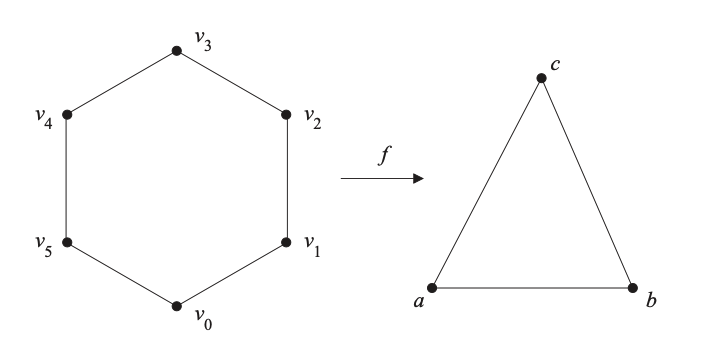
\includegraphics[scale = 0.25]{pictures/exemplefinalhomologiasimplicial.png}
    \caption{Exemple d'aplicacions simplicial.}
    \label{fig:exemplefinalhomologiasimplicial}
\end{figure}

Com $|K|$ i $|L|$ són connexos, es té $H_0(K)\cong \mathbb{Z}$ i $H_0(L)\cong \mathbb{Z}$, i a més aquests grups estan generats per un vèrtex qualsevol dels respectius políedres. Així, en resulta que $f$ indueix un isomorfisme $H_0(K)\cong H_0(L)$.

Respecte a l'acció de $f$ en els grups $H_1$, observem que $H_1(K)\cong\mathbb{Z}$ està generat per la classe del cicle
\begin{equation}
    \notag
    z = [v_0,v_1]+[v_1,v_2]+[v_2,v_3]+[v_3,v_4]+[v_4,v_5]-[v_0,v_5],
\end{equation}
i que $H_1(L)\cong\mathbb{Z}$ està generat per la classe del cicle
\begin{equation}
    \notag
    z' = [a,b]+[b,c]-[a,c].
\end{equation}
És immediat comprovar que $f_\bullet(z) = 2z'$. Així, a través dels isomorfismes $H_1(K) = Z[z]\cong\mathbb{Z}$ i $H_1(L) = \mathbb{Z}[z']\cong \mathbb{Z}$, el morfisme induït en $H_1$,
\begin{equation}
    \notag
    H_1(K)\longrightarrow H_1(L)
\end{equation}
correspon a la multiplicació per 2. Aquesta acció té un significat geomètric clar, ja que mentre donem una volta a $K$, la imatge dona dues voltes a $L$. Més endavant veurem que l'enter 2 és el grau de $f$.










\section{Homotopies entre morfismes de complexos de \texorpdfstring{$R$}{TEXT}-mòduls}

Aquest apartat el copiaré gairebé al peu de la lletra dels apunts que algune bone samaritane ha penjat al drive, ja que a classe s'ha donat però en un altre ordre i més endavant, traient-lo de context i, per tant, no m'he enterat de res. 

En aquest apartat introduirem la noció d'homotopia entre morfismes de complexos de $R$-mòduls. Aquesta noció es pot pensar com l'anàleg algebraic de la noció d'homotopia entre aplicacions contínues.

\begin{defi}
Siguin $M_\bullet$ i $M_\bullet'$ dos complexos de cadenes de $R$-mòduls, i $f,g:M_\bullet\rightarrow M_\bullet'$ dos morfismes de complexos. Es diu que $f$ i $g$ són \textit{morfismes homòtops}\index{Morfismes homòtops} si existeix una successió de morfismes de $R$-mòduls $\{h_p\}_p$ tal que $h_p:M_p\rightarrow M_{p+1}'$, $p\geq 0$, tal que, considerant $h_{-1} = 0$, es verifica   
\begin{equation}
    \notag
    f_p-g_p = \partial_{p+1}h_p+h_{p-1}\partial_p,
\end{equation}
per a tot $p\geq0$. Direm que $h$ és una \textit{homotopia} entre els morfismes $f$ i $g$.
\end{defi}

El diagrama següent recull la informació que proporciona una homotopia entre els morfismes $f$ i $g$:
\begin{equation}
    \notag
    \xymatrix@=3em{
    \cdots \ar[r] & M_{p+2}\ar[r]^{\partial_{p+2}}\ar@<-.5ex>[d]_f\ar@<.5ex>[d]^g & M_{p+1}\ar[r]^{\partial_{p+1}}\ar@<-.5ex>[d]_f\ar@<.5ex>[d]^{g_{p+1}}\ar[dl]^h & M_p\ar[r]^{\partial_p}\ar@<-.5ex>[d]_{f_p}\ar@<.5ex>[d]^{g_p}\ar[dl]^{h_p} & M_{p-1}\ar[r]\ar@<-.5ex>[d]_f\ar@<.5ex>[d]^g\ar[dl]^h & \cdots \\
    \cdots \ar[r] & M_{p+2}'\ar[r]^{\partial_{p+2}'} & M_{p+1}'\ar[r]^{\partial_{p+1}'} & M_p'\ar[r]^{\partial_p'} & M_{p-1}'\ar[r] & \cdots
    }
\end{equation}

En aquest diagrama s'han de verificar les commutativitats expressades per les igualtats de la definició. Una primera mostra de l'interès d'aquesta definició ve donada pel següent resultat.

\begin{prop}
Si $f,g:M_\bullet\rightarrow M_\bullet'$ són morfismes homòtops de complexos de $R$-mòduls, llavors indueixen el mateix morfisme en homologia,
\begin{equation}
    \notag
    H_\bullet(f) = H_\bullet(g):H_\bullet(M_\bullet)\rightarrow H_\bullet(M_\bullet').
\end{equation}
\end{prop}
\begin{proof}
Prenem una classe $[z]\in H_n(M_\bullet)$, representada per $z\in Z_n(M_\bullet)$, que, en ser un cicle, verifica $\partial_n(z) = 0$. Llavors, $H_\bullet(f)[z]$ està representada per $f(z)\in Z_n(M_\bullet')$, mentre que $H_\bullet(g)[z]$ està representada per $g(z)\in Z_n(M_\bullet')$, i per la definició d'homotopia
\begin{equation}
    \notag
    f(z)-g(z) = h(\partial(z))+\partial(h(z)) = \partial(h(z)),
\end{equation}
per tant,
\begin{equation}
    \notag
    f(z)-g(z)\in B_n(M_\bullet')
\end{equation}
d'on resulta que les classes són iguals en $H_n(M_\bullet')$.
\end{proof}













\end{document}